\documentclass[landscape,9pt]{beamer}

%% define basic beamer themes 
\usetheme{Boadilla}
\usecolortheme{whale} 
\usefonttheme[onlymath]{serif}

% Settings for tikz (to make graphs)
\usepackage{tikz,verbatim,graphicx}
\usetikzlibrary{shapes,arrows,arrows.meta,decorations.pathreplacing,positioning}

%%%%%%% creates logs
\newcommand{\MRC}{
\logo{
\includegraphics[height=.37cm]{MRC.png}} 
\setbeamertemplate{sidebar right}{% 
  \vfill%
  \llap{\insertlogo\hskip0.0cm}%
}
}

\newcommand{\UCL}{
\logo{
\includegraphics[height=.37cm]{UCL.jpg}} 
\setbeamertemplate{sidebar right}{% 
  \vfill%
  \llap{\insertlogo\hskip0.0cm}\vskip0.015cm%
}
}

\newcommand{\Bristol}{
\logo{
\includegraphics[height=.37cm]{Bristol.png}}
\setbeamertemplate{sidebar right}{% 
  \vfill%
  \llap{\insertlogo\hskip0.02cm}\vskip0.02cm%
}
}

\newcommand{\Sheffield}{
\logo{\includegraphics[height=.39cm]{Sheffield.jpg}}
\setbeamertemplate{sidebar right}{% 
  \vfill%
  \llap{\insertlogo\hskip0.0cm}\vskip0.015cm%
}
}

\newcommand{\Sickkids}{
\logo{\includegraphics[height=.39cm]{Sickkids.png}}
\setbeamertemplate{sidebar right}{% 
  \vfill%
  \llap{\insertlogo\hskip0.0cm}\vskip0.015cm%
}
}

\newcommand{\nologo}{
\logo{}
}

%%%%\setbeamerfont{structure}{size=\fontsize{10}{11}\selectfont}

%% This creates a counter to get the first & last frame of each part
%% source: http://tex.stackexchange.com/questions/73142/how-can-i-get-the-first-and-the-last-frame-of-an-part-in-beamer-class
\usepackage{etoolbox}
\makeatletter
\newcount\beamer@partstartframe
\beamer@partstartframe=1
\apptocmd{\beamer@part}{\addtocontents{nav}{\protect\headcommand{%
        \protect\beamer@partframes{\the\beamer@partstartframe}{\the\c@framenumber}}}}{}{}
\apptocmd{\beamer@part}{\beamer@partstartframe=\c@framenumber\advance\beamer@partstartframe by1\relax}{}{}
\AtEndDocument{\immediate\write\@auxout{\string\@writefile{nav}%
        {\noexpand\headcommand{\noexpand\beamer@partframes{\the\beamer@partstartframe}{\the\c@framenumber}}}}}{}{}
\def\beamer@startframeofpart{1}
\def\beamer@endframeofpart{1}
\def\beamer@partframes#1#2{%
  \ifnum\c@framenumber<#1%
  \else%
    \ifnum\c@framenumber>#2%
    \else%
      \gdef\beamer@startframeofpart{#1}%
      \gdef\beamer@endframeofpart{#2}%
    \fi%
  \fi%
}
\newcommand\insertpartstartframe{\beamer@startframeofpart}
\newcommand\insertpartendframe{\beamer@endframeofpart}
\makeatother

%%% include replacement file beamerbaseframe.sty in working dir - 
%%% fixes bug with wrong frame number for fragile slides.
\usepackage{beamerbaseframe}

\PassOptionsToPackage{pdftex,usenames,dvipsnames}{color}
\bibliographystyle{unsrt}
\usepackage{amssymb,amsmath,multirow,colortbl,graphics,bm,inconsolata,marvosym}
%\usepackage[T1]{fontenc}
\usepackage[normalem]{ulem}
\usepackage[abs]{overpic}		% Allows over pictures in frame
%\usepackage{times}
\usepackage{xspace} %% solves space annoyance with \winbugs macro
\usepackage{pstricks}
\usepackage[position=top]{subfig}
\usepackage{animate,framed,tabto,verbatim}
\usepackage{inputenc}
\usepackage{graphicx,mathrsfs,bibentry,chngcntr,booktabs,fancyvrb}
\usepackage[authoryear]{natbib}
%%%\usepackage{url}

% To format computer code
\usepackage{listings}
\lstset{basicstyle=\ttfamily\fontsize{6}{7}\selectfont,breaklines=true,tabsize=2,
keywords={},linewidth=1\textwidth,backgroundcolor=\color{black!5}} 

\raggedright %no right-justify
\setlength{\parskip}{3pt}

\newenvironment{shitemize}{\begin{itemize}
\setlength{\parskip}{0pt}
\setlength{\itemsep}{2pt}
\setlength{\parsep}{0pt}
}{\end{itemize}}

\newcommand{\Sum}{\displaystyle \sum}
\newcommand{\bi}{\begin{itemize}}
\newcommand{\ei}{\end{itemize}}

\newcommand{\winbugs}{{\texttt{WinBUGS}}\xspace}
\newcommand{\openbugs}{{\texttt{OpenBUGS}}\xspace}
\newcommand{\jags}{{\texttt{JAGS}}\xspace}
\newcommand{\bugs}{{\texttt{BUGS}}\xspace}

\newcommand{\tca}[1]{\textcolor{black}{#1}}
\newcommand{\tcb}[1]{\textcolor{black}{#1}}

\newcommand{\bpi}{\mbox{\boldmath $ \pi $}}
\newcommand{\bLambda}{\mbox{\boldmath $ \Lambda $}}
\newcommand{\bc}{\mbox{\boldmath $ c $}}
\newcommand{\bb}{\mbox{\boldmath $ b $}}
\newcommand{\bC}{\mbox{\boldmath $ C $}}

\newcommand{\distspace}{ \,\,\,\,\,}
\newcommand{\ie}{ {\hspace{-1.5mm}\it i.e.} }
\newcommand{\eg}{ {\hspace{-1.5mm}\it e.g.} }

\newcommand{\EXP}{\ensuremath{\mathbb{E}}}
\newcommand{\VAR}{\ensuremath{\mathbb{V}}}
\newcommand{\COV}{\ensuremath{\mathbb{V}}}
%\newcommand{\E}{\mbox{\boldmath $ E $}}
\newcommand{\E}{\mbox{E}}

\newcommand{\pd}[1]{\parbox[c]{1.2 cm}{\fontsize{6}{5} \selectfont \centering #1}}
\newcommand{\ps}[1]{\parbox[c]{1 cm}{\fontsize{6}{5} \selectfont \centering #1}}
\renewcommand{\b}{\mbox{B}}
\newcommand{\bcea}{\texttt{BCEA}\xspace}
\newcommand{\R}{\texttt{R}\xspace}
\newcommand{\hs}{\hspace{5pt}}
\newcommand{\mytilde}{{\raise.17ex\hbox{$\scriptstyle\mathtt{\sim}$}}\xspace}
\newcommand{\logit}{\mathop{\mathrm{logit}}}

\newcommand{\bx}{\mbox{$\mathbf{x}$}}
\newcommand{\xvec}{\mbox{$\bx_1,\ldots,\bx_n$}}
\newcommand{\yxvec}{\mbox{$y_1=f(\bx_1),\ldots,y_n=f(\bx_n)$}}
\newcommand{\by}{\mbox{$\mathbf{y}$}}
\newcommand{\bh}{\mbox{$\mathbf{h}$}}
\newcommand{\bt}{\mbox{$\mathbf{t}$}}
\newcommand{\bbeta}{\mbox{\boldmath{$\beta$}}\unboldmath}
\newcommand{\bdelta}{\mbox{\boldmath{$\delta$}}\unboldmath}
\newcommand{\bphi}{\mbox{\boldmath{$\phi$}}\unboldmath}
\newcommand{\btheta}{\mbox{\boldmath{$\theta$}}\unboldmath}
\newcommand{\bo}[1]{\mbox{$\mathbf{#1}$}}
\newcommand{\yxpvec}{\mbox{$y_1'=\eta(\bx_1'),\ldots,y_{n'}'=\eta(\bx_{n'}')$}}
\newcommand{\xpvec}{\mbox{$\bx_1',\ldots,\bx_{n'}'$}}
\newcommand{\ri}{\mbox{$^{131}I$} }
\newcommand{\bZ}{\mbox{$\bm{Z}$}}
\newcommand{\T}{\mbox{$\bm{\theta}$}}
\newcommand{\X}{\mbox{$\bm{X}$}}
\newcommand{\x}{\mbox{$\bm{x}$}}
%\newcommand{\btheta}{\mbox{$\bm{\theta}$}}
\newcommand{\M}{\mbox{$\NB(d,\bm\theta)$}}
\newcommand{\NB}{\mbox{NB}}
\newcommand{\nb}{\mbox{$\mathbf{nb}$}}
\newcommand{\EVPI}{\mbox{$\mbox{EVPPI}$}}
\newcommand{\EVSI}{\mbox{EVSI}}
\newcommand{\Cov}{\mbox{$\mbox{Cov}$}}
\newcommand{\bX}{\mbox{$\bm{X}$}}
\newcommand{\K}{\mbox{$\mathbf{K}$}}
\newcommand\independent{\protect\mathpalette{\protect\independenT}{\perp}}
\def\independenT#1#2{\mathrel{\rlap{$#1#2$}\mkern4mu{#1#2}}}
\newcommand{\notindependent}{%
\mathrel{\ooalign{$\independent$\cr\kern3pt$/$}}}
\newcommand{\Data}{%
\mathrm{Data}}
\newcommand{\dd}{%
\mathrm{d}}
\newcommand{\N}{\mbox{${NB}$}}

\newenvironment{shenumerate}{\begin{enumerate}
\setlength{\parskip}{0pt}
\setlength{\itemsep}{2pt}
\setlength{\parsep}{0pt}
}{\end{enumerate}}

%% Books to reference
\newcommand{\bmhe}{\footnotesize  \textit{Bayesian Methods in Health Economics: Day 2 Practical}}
\newcommand{\bugsbook}{\footnotesize  \textit{The \texttt{BUGS} Book}}
\newcommand{\bceabook}{\footnotesize  Baio et al (2017). \textit{Bayesian Cost-Effectiveness Analysis with the \texttt{R} package \texttt{BCEA}}}
\newcommand{\esdmh}{\footnotesize Welton et al (2012). \textit{Evidence Synthesis for Decision Making in Healthcare}}
\newcommand{\gelmanhill}{\footnotesize Gelman and Hill (2007). \textit{Data Analysis Using Regression and Multilevel/Hierarchical Models}}

\definecolor{rpurple}{rgb}{0.627, 0.125, 0.941}
\setbeamerfont{alerted text}{shape=\itshape}
\setbeamerfont{local structure}{shape=\slshape}
\setbeamercolor{alerted text}{fg=rpurple!80!black}
\setbeamercolor{alerted text}{fg=rpurple!80!black}

%% Defines a few new colors and commands to use them easily
\definecolor{myblue}{rgb}{0.14, 0.34, 0.55}
\definecolor{orange}{rgb}{1, 0.5, 0}
\definecolor{olive}{rgb}{.2, .31, .09}
\newcommand{\myblue}{\color{myblue}}
\newcommand{\orange}{\color{orange}}
\newcommand{\olive}{\color{olive}}
\renewcommand{\red}{\color{red}}
\renewcommand{\blue}{\color{blue}}
\renewcommand{\black}{\color{black}}
\renewcommand{\white}{\color{white}}
\renewcommand{\gray}{\color{gray}}
\newrgbcolor{amber}{1.0, 0.75, 0.0}
\definecolor{darkgrey}{rgb}{.83 .83 .83}
\newcommand\darkgrey{\color{darkgrey}}

\usepackage{hyperref}
\hypersetup{colorlinks=true,urlcolor=myblue,linkcolor=}

\setbeamertemplate{navigation symbols}{}

\setbeamerfont{footnote}{size=\tiny}
\addtobeamertemplate{footnote}{}{\vspace{1ex}}

\setbeamerfont{itemize/enumerate body}{size*={9}{11}}
\setbeamerfont{itemize/enumerate subbody}{size*={8}{10}}
\setbeamerfont{itemize/enumerate subsubbody}{size*={7}{9}}


% make all itemizes appear one point by one. 
% don't put this in, doubles the file size 
% \beamerdefaultoverlayspecification{<+->}

\title{Bayesian Methods in Health Economics: Day 2 Practical}
\part{Stockholm, Sweden}
\date{9-10th June 2022}
\author{Nathan Green (n.green@ucl.ac.uk)\\
(with thanks to Gianluca Baio, Chris Jackson, Nicky J.~Welton, Mark Strong, Anna Heath)}

\begin{document}
\frame{\titlepage}

\date{Day 1}

\addtocounter{part}{-1}			% Labels the first part as 0 --- preliminaries
\renewcommand{\partname}{ }		% Remove the label "Part"
%% customised footline for the preliminaries
\makeatletter
\setbeamertemplate{footline}{%
  \leavevmode%
  \hbox{%
  \begin{beamercolorbox}[wd=.35\paperwidth,ht=2.25ex,dp=1ex,center]{title in head/foot}%
    \usebeamerfont{title in head/foot}\insertshorttitle
  \end{beamercolorbox}%
  \begin{beamercolorbox}[wd=.10\paperwidth,ht=2.25ex,dp=1ex,center]{date in head/foot}% original wd=.15
    \usebeamerfont{date in head/foot}\insertshortdate{}
  \end{beamercolorbox}%
  \begin{beamercolorbox}[wd=.40\paperwidth,ht=2.25ex,dp=1ex,center]{section in head/foot}% original wd=.35
    \usebeamerfont{section in head/foot} \insertshortpart 
  \end{beamercolorbox}%
  \begin{beamercolorbox}[wd=.15\paperwidth,ht=2.25ex,dp=1ex,center]{date in head/foot}%
%    \insertframenumber{}\hspace*{1ex}(\insertpartstartpage--\insertpartendpage)
%    \insertframenumber{}\hspace*{1ex}(\insertpartstartframe--\insertpartendframe)
  \end{beamercolorbox}}%
  \vskip0pt%
}
\makeatother
\part[Preliminaries]{Preliminaries} \frame{\partpage} 

\begin{frame}
\frametitle{University College London}
\begin{tabular}{lcr}
\begin{minipage}[l]{5.0cm}
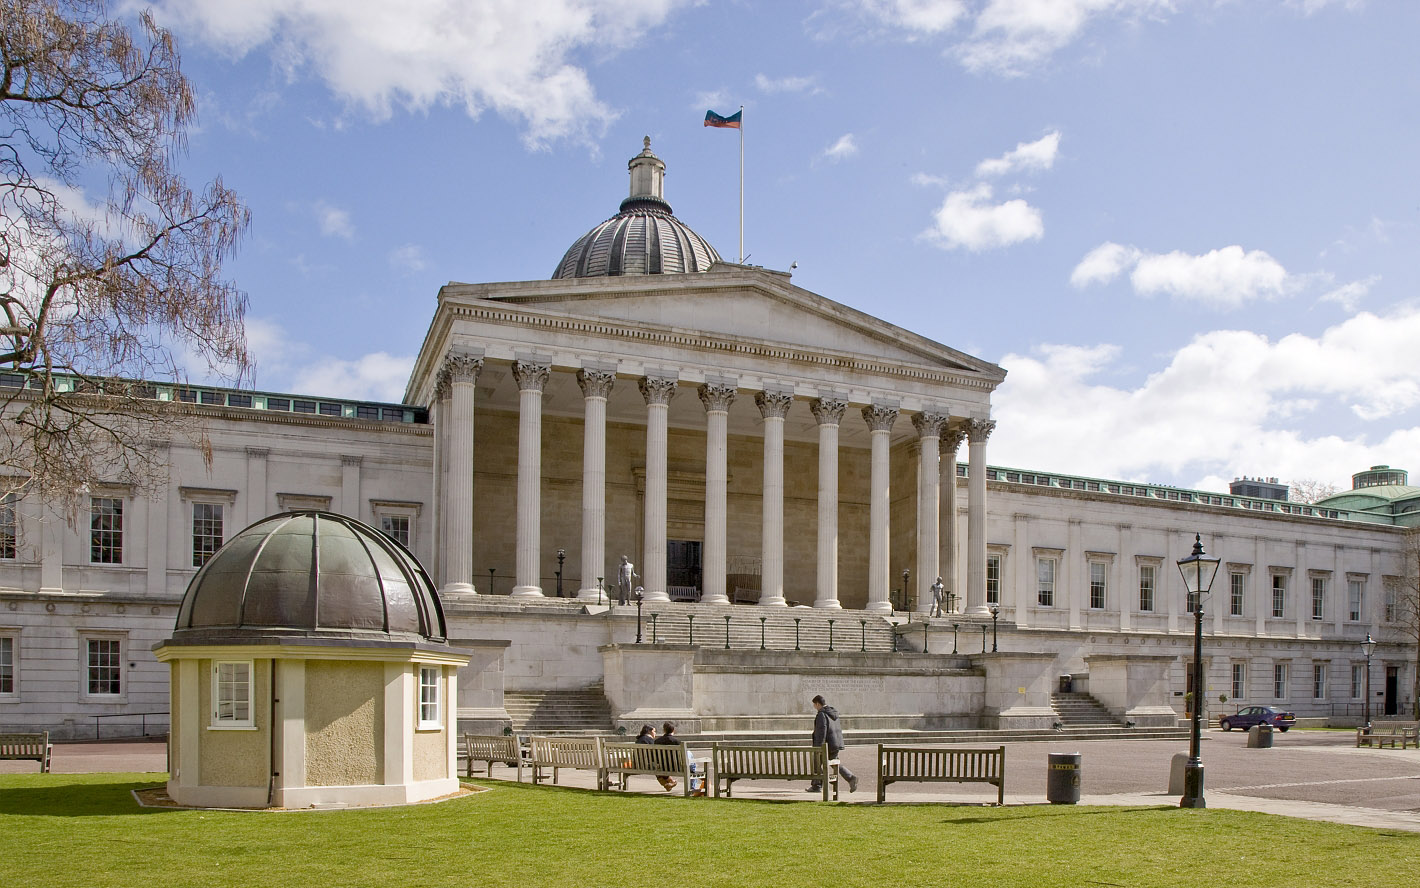
\includegraphics[height=3.8cm]{ucl_building}
\end{minipage} & &
\begin{minipage}[r]{6.5cm}
\begin{itemize}
\item UCL was rated 2nd in the UK for research power in the Research Excellence Framework 2021
\item UCL is ranked 8th in the 2022 QS World University Rankings
\item The Department of Statistical Science has played a major role in the development of the subject ever since its foundation in 1911 as the Department of Applied Statistics
\end{itemize}
\end{minipage}
\end{tabular}
\end{frame}

\begin{frame}%[noframenumbering]
\frametitle{Objectives}

\only<1>{
\begin{tabular}{lcr}
\begin{minipage}[l]{5.0cm}
\textbf{Lectures}\\
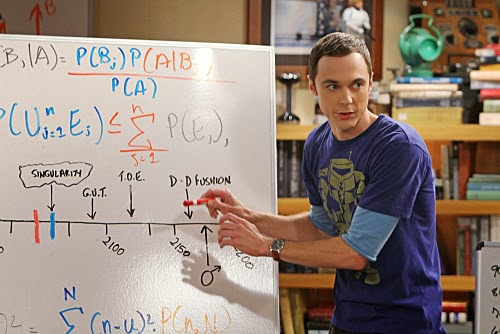
\includegraphics[height=3.8cm]{Lecture}
\end{minipage} & &
\begin{minipage}[r]{6.5cm}
\begin{itemize}
	\item Introduction to \alert{Health economics modelling}
	\begin{itemize}
		\item Decision trees
		\item Markov models
	\end{itemize}
	\vspace{10pt}
	\item Introduction to sensitivity analyses
	\begin{itemize}
		\item Deterministic
		\begin{itemize}
			\item One-way \& multi-way
			\item Scenario
		\end{itemize}
		\item Probabilistic
	\end{itemize}  
\end{itemize}
\end{minipage}
\end{tabular}}

\only<2>{
\begin{tabular}{lcr}
\begin{minipage}[l]{5.0cm}
\textbf{Computer practicals}\\
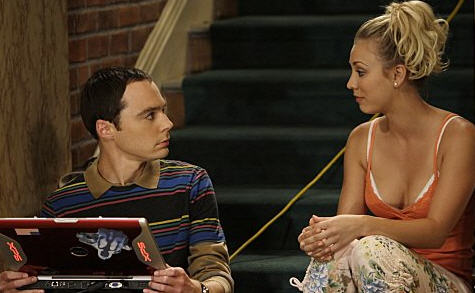
\includegraphics[height=3.5cm]{Practical}
\end{minipage} & &
\begin{minipage}[r]{6.5cm}
\begin{itemize}
\item Emphasis on practical examples
\begin{itemize}
\item Decision tree and Markov models 
\item using \texttt{R} programming language
\end{itemize}
\end{itemize}
\end{minipage} 
\end{tabular}}
\end{frame}

\frame{
\frametitle{Timetable}
\begin{itemize}
\item 2:00-3:00 Health Economics modelling lecture
\item 3:00 - 3:45 Decision tree and Markov model practical
\item BREAK
\item 3:50 - 4:20 Sensitivity analysis lecture
\item 4:20-5:00 Sensitivity analysis practical
\end{itemize}
}

\begin{frame}%[noframenumbering]
\frametitle{More Bayesian Health Economics...}

\begin{tabular}{lcr}
\begin{minipage}[l]{5.0cm}
\textbf{Books}\\

\includegraphics[height=3.8cm]{bcea_book}
\includegraphics[height=3.8cm]{bmhe_book}
\end{minipage} & &
\begin{minipage}[r]{6.5cm}
\begin{itemize}
\item This course is only a small part of an \alert{annual week-long summer school}
\begin{itemize}
\item usually in Florence, Italy
\end{itemize}
\item Several books available
\item Edition two of BCEA book in the pipeline and a Health Economic in R book close to being finished!
\end{itemize}

\end{minipage}
\end{tabular}
\end{frame}



% This changes the default setting and uses arabic instead of Roman numbers for the parts (lectures)
% source: https://tex.stackexchange.com/questions/65560/changing-of-the-numbering-of-parts-in-beamer
\setbeamertemplate{part page}
{
  \begin{centering}
    {\usebeamerfont{part name}\usebeamercolor[fg]{part name}\partname~\insertpartnumber}
    \vskip1em\par
    \begin{beamercolorbox}[sep=10pt,center,rounded=true]{part title}
      \usebeamerfont{part title}\insertpart\par
    \end{beamercolorbox}
  \end{centering}
}
%% customised footline (same as before but now also includes the lecture number in the footer
\makeatletter
\setbeamertemplate{footline}{%
  \leavevmode%
  \hbox{%
  \begin{beamercolorbox}[wd=.35\paperwidth,ht=2.25ex,dp=1ex,center]{title in head/foot}%
    \usebeamerfont{title in head/foot}\insertshorttitle
  \end{beamercolorbox}%
  \begin{beamercolorbox}[wd=.10\paperwidth,ht=2.25ex,dp=1ex,center]{date in head/foot}% original wd=.15
    \usebeamerfont{date in head/foot}\insertshortdate{}
  \end{beamercolorbox}%
  \begin{beamercolorbox}[wd=.40\paperwidth,ht=2.25ex,dp=1ex,center]{section in head/foot}% original wd=.35
    \usebeamerfont{section in head/foot} \insertpartnumber.\ \insertshortpart 
  \end{beamercolorbox}%
  \begin{beamercolorbox}[wd=.15\paperwidth,ht=2.25ex,dp=1ex,center]{date in head/foot}%
%    \insertframenumber{}\hspace*{1ex}(\insertpartstartpage--\insertpartendpage)
    \insertframenumber{}\hspace*{1ex}(\insertpartstartframe--\insertpartendframe)
  \end{beamercolorbox}}%
  \vskip0pt%
}
\makeatother

\renewcommand{\partname}{Lecture}	% Changes the label "Part" to "Lecture"
\addtocounter{framenumber}{-3}


%% customised footline for the final slide
\makeatletter
\setbeamertemplate{footline}{%
  \leavevmode%
  \hbox{%
  \begin{beamercolorbox}[wd=.35\paperwidth,ht=2.25ex,dp=1ex,center]{title in head/foot}%
    \usebeamerfont{title in head/foot}\insertshorttitle
  \end{beamercolorbox}%
  \begin{beamercolorbox}[wd=.10\paperwidth,ht=2.25ex,dp=1ex,center]{date in head/foot}% original wd=.15
    \usebeamerfont{date in head/foot}\insertshortdate{}
  \end{beamercolorbox}%
  \begin{beamercolorbox}[wd=.40\paperwidth,ht=2.25ex,dp=1ex,center]{section in head/foot}% original wd=.35
    \usebeamerfont{section in head/foot} \insertshortpart 
  \end{beamercolorbox}%
  \begin{beamercolorbox}[wd=.15\paperwidth,ht=2.25ex,dp=1ex,center]{date in head/foot}%
%    \insertframenumber{}\hspace*{1ex}(\insertpartstartpage--\insertpartendpage)
    \insertframenumber{}\hspace*{1ex}(\insertpartstartframe--\insertpartendframe)
  \end{beamercolorbox}}%
  \vskip0pt%
}


\end{document}

